\iflanguage{ngerman}
{\chapter{Methoden und Umsetzung}}
{\chapter{Methods and Implementation}}
\label{sec:methods}

\section{Einbindung in das Framework}
%\par\setlength{\parindent}{10pt}
Die Plot-Demo wird mit dem Plugin-Interface des CGVF implementiert.
Dieses Plugin kann dann von der Viewer Anwendung aufgerufen werden.
Das Plugin wird dabei von einer Hauptklasse repräsentiert, diese nutzt das Node-Interface des Frameworks.
Wird das Plugin aufgerufen, wird auch der Konstruktor der Klasse aufgerufen.
\par%\setlength{\parindent}{10pt}
Zudem nutzt das Plugin das Render-Interface, das die Methoden 'init' und 'draw' zur Verfügung stellt.
Dieses Interface macht es möglich eine Interne Render-Pipeline vom Framework zu nutzen, sodass am Ende nur die Shader modifiziert werden müssen.
Die Methode 'init' wird vor dem Rendern des ersten Frames aufgerufen und die 'draw' Methode beim Rendern jedes Frames.
\par
Zuletzt nutzt das Plugin das GUI-Interface, das die Erstellung einer einfachen Nutzeroberfläche aus vorgefertigten Elementen in der Viewer Anwendung ermöglicht.
\begin{figure}[ht]
	\begin{lstlisting}[language=C++]
class procedural_plot :
        public cgv::base::node,
        public cgv::render::drawable,
        public cgv::gui::provider {
...
bool init(cgv::render::context &ctx) override { ... }
...
void draw(cgv::render::context &ctx) override { ... }
...
void create_gui() override { ... }
... }
	\end{lstlisting}
	\caption{procedural\_plot.cxx Plugin Aufbau}
	\label{fig:code_plugin}
\end{figure}



\section{Rectangle-Renderer}
Der Rectangle-Renderer (RCR) ist eine Hilfsklasse des CGVF, zur Darstellung einer einfachen Rechteckgeometrie.
Dieser hat bereits ein vorgegebenes Shader-Programm, dass heißt es müssen nur noch Position und Dimension des Rechtecks angegeben werden und der RCR kann das Rechteck in der 'draw' Methode darstellen.
In Abbildung \ref{fig:code_rcr} wird statt dem Vorgabeprogramm ein eigenes Shader-Programm genutzt, das die Funktionalität zur Darstellung der Plots enthalten wird.
\begin{figure}[ht]
	\begin{lstlisting}[language=C++]
auto &rcr = cgv::render::ref_rectangle_renderer(ctx, 0);
rcr.set_prog(shader_program);
rcr.set_position(ctx, RECT_POSITION);
rcr.set_extent(ctx, RECT_EXTEND);
rcr.render(ctx, 0, 1);
	\end{lstlisting}
	\caption{procedural\_plot.cxx Rectangle-Renderer}
	\label{fig:code_rcr}
\end{figure}



\section{Shader-Programm}
Ein Shader-Programm im CGVF ist eine Sammlung von allen Shadern in der Shader-Pipeline die zum Darstellen einer Szene im Viewer gebraucht werden.
Mit einer 'glpr' Datei werden alle Teildateien des Shader-Programms definiert.
In Abbildung \ref{fig:code_sp2} wird die 'rectangle.glpr' Datei, das Vorgabeprogramm auf dem RCR, als Grundlage genutzt und um die Dateien 'sdf.glfs' und 'procedural\_plot.glfs' erweitert.
\begin{figure}[ht]
	\begin{lstlisting}
files:rectangle
vertex_file:group.glsl
vertex_file:quaternion.glsl
vertex_file:view.glsl
geometry_file:side.glsl
geometry_file:view.glsl
fragment_file:sdf.glfs
fragment_file:procedural_plot.glfs
fragment_file:side.glsl
fragment_file:lights.glsl
fragment_file:bump_map.glfs
fragment_file:surface.glsl
fragment_file:brdf.glsl
	\end{lstlisting}
	\caption{procedural\_plot.glpr}
	\label{fig:code_sp2}
\end{figure}
\par
Mit der Member-Funktion 'build\_program' werden in der Abbildung \ref{fig:code_sp1} alle, in der 'glpr' definierten Shader-Dateien kompiliert und dem Shader-Programm hinzugefügt.
\begin{figure}[ht]
	\begin{lstlisting}[language=C++]
cgv::render::shader_program shader_program;
shader_program.build_program(ctx, "procedural_plot.glpr", true, defines);
	\end{lstlisting}
	\caption{procedural\_plot.cxx Shader-Programm Erstellung}
	\label{fig:code_sp1}
\end{figure}



\section{Übermittlung an den Shader}
Da sich der Kern der Implementation für die Plot-Darstellung im Fragment-Shader befindet, muss es einen Weg geben, die Eingaben aus dem Nutzer-Interface und die Graph-Daten in den Shader zu laden, um sie dort nutzen zu können.
Für diesen Zweck werden tatsächlich drei verschiedene Wege genutzt: Compiler-Defines, Uniform-Variablen und Shader-Storage-Buffer.

\subsection{Compiler-Defines}
Compiler-Defines im Shader werden hier genutzt, um bestimmte Teile des Codes nur dann zu, wenn ein Define gesetzt ist.
Dadurch können verschachtelte If-Statements vermieden und so Performance gespart werden.
Zudem können Defines auch genutzt werden um einfache Integer-Werte zu übermitteln, die nur beim erneuten bauen des Shaders aktualisiert werden müssen.
Wenn im Shader eine Funktion aktiviert oder deaktiviert werden soll, dann wird in Abbildung \ref{fig:code_cd1} der Define gesetzt oder nicht gesetzt und das Shader-Programm wird neu gebaut.
\begin{figure}[ht]
	\begin{lstlisting}[language=C++]
bool is_hidden = false;
const cgv::render::shader_define_map defines = {
            {"IS_HIDDEN",    std::to_string(is_hidden)}
};
if (defines != current_defines) {
        shader_program.destruct(ctx);
        shader_program.build_program(ctx, "procedural_plot.glpr", true, defines);
        current_defines = defines;
}
	\end{lstlisting}
	\caption{procedural\_plot.cxx Compiler-Defines werden gesetzt}
	\label{fig:code_cd1}
\end{figure}
\par
Im Shader muss zunächst der Default-Define gesetzt werden, damit der Compiler weiß, dass dieser Define existiert.
In Abbildung \ref{fig:code_cd2} werden die Bereiche des Codes zwischen '\#if ...' und '\#endif' abhängig vom Define geladen oder nicht geladen.
\begin{figure}[ht]
	\begin{lstlisting}[language=GLSL]
#define IS_HIDDEN 0
color = vec4(vec3(0.3), 1.0);
#if IS_HIDDEN == 1
color.a = 0.0f;
#endif
frag_color = color;
	\end{lstlisting}
	\caption{procedural\_plot.glfs Compiler-Defines im Shader}
	\label{fig:code_cd2}
\end{figure}
\FloatBarrier

\subsection{Uniform-Variablen}
Uniform-Variablen werden genutzt um Konfigurationsdaten an den Shader zu senden, die nicht mit einem einfachen ja/nein ausgedrückt werden können, bzw. häufiger aktualisiert werden müssen.
Es können auch Arrays mit Festgröße bzw. Vektoren übermittelt werden.
\begin{figure}[ht]
	\begin{lstlisting}[language=C++]
template<typename T>
void set_uniform(cgv::render::context &ctx, const std::basic_string<char> &name, const T &value) {
    shader_program.set_uniform(ctx, shader_program.get_uniform_location(ctx, name), value);
}

set_uniform(ctx, "alpha_test_val", domain_alpha);
set_uniform(ctx, "domain_extent", RECT_EXTEND);
	\end{lstlisting}
	\caption{procedural\_plot.cxx Setzen zweier Uniform-Variablen}
	\label{fig:code_uv1}
\end{figure}
\begin{figure}[ht]
	\begin{lstlisting}[language=GLSL]
uniform float alpha_test_val;
uniform vec2 domain_extent;
	\end{lstlisting}
	\caption{procedural\_plot.glfs Definition der Uniform-Variablen im Shader}
	\label{fig:code_uv2}
\end{figure}
\FloatBarrier

\subsection{Shader-Storage-Buffer}
Shader-Storage-Buffer (abgekürzt mit SSB) sind Buffer mit einer nicht vordefinierten Größe die unabhängig von den Uniform-Variablen aktualisiert werden können.
Durch die dynamische Größe bieten sich SSBs an, um die vollständigen Graph-Daten in Sets in den Shader zu laden.
Ein SSB lädt dabei alle Daten von beliebig vielen Graphen, sequenziell aneinander gereiht.
Ein zweiter SSB lädt zusätzliche die Anzahl der Datenpaare, die Färbung des  Graphen und die Skalierung des Graphen als Parameter für jeden Graphen, ebenfalls sequenziell aufgereiht.
Diese Parameter sind in dem Struct 'Graph\_Param' definiert.
Das CGVF bietet bereits implementierte SSBs an.
In Abbildung \ref{fig:code_sb1} wird die vordefinierte Klasse 'vertex\_buffer' genutzt.
\begin{figure}[ht]
	\begin{lstlisting}[language=C++]
cgv::render::vertex_buffer vec_sbo, segment_sbo;
std::vector<cgv::math::fvec<float, 2>> graph_data;
std::vector<Graph_Param> graph_param;

template<typename T>
void load_data_buffer(cgv::render::context &ctx, cgv::render::vertex_buffer &buffer, T &data) {
    cgv::render::vertex_buffer sbo(cgv::render::VBT_STORAGE, cgv::render::VBU_STATIC_READ);
    if (!sbo.create(ctx, data)) throw;
    buffer = std::move(sbo);
}

segment_sbo.destruct(ctx);
vec_sbo.destruct(ctx);
load_data_buffer(ctx, segment_sbo, graph_param);
load_data_buffer(ctx, vec_sbo, graph_data);

const int vec_sbo_h = vec_sbo.handle ? (const int &) vec_sbo.handle - 1 : 0,
                      segment_sbo_h = segment_sbo.handle ? (const int &) segment_sbo.handle - 1 : 0;
glBindBufferBase(GL_SHADER_STORAGE_BUFFER, 0, segment_sbo_h);
glBindBufferBase(GL_SHADER_STORAGE_BUFFER, 1, vec_sbo_h);
	\end{lstlisting}
	\caption{procedural\_plot.cxx Erstellen und Binden von SSBs}
	\label{fig:code_sb1}
\end{figure}
\begin{figure}[ht]
	\begin{lstlisting}[language=GLSL]
struct Graph_Param
{
	int vertex_count;
	float color[4];
	float scale[2];
};

layout(std430, binding = 0) readonly buffer GP { Graph_Param graph_param[]; };
layout(std430, binding = 1) readonly buffer GD { vec2 graph_data[]; };
	\end{lstlisting}
	\caption{procedural\_plot.glfs Definition von SSBs im Shader}
	\label{fig:code_sb2}
\end{figure}
\FloatBarrier


\section{SDF-Implementationen}
Alle SDFs sind in einer eigenen Shader-Datei 'sdf.glfs'.
Diese SDFs stammen aus Artikeln von Inigo Quilez \cite{Inigo}, da seine Implementationen die effizientesten sind, die ich gefunden habe.
Effizient bedeutet hier die wenigsten Instruktionen des kompilierten Shaders auf der Grafikkarte.
In Abbildung \ref{fig:code_sdf1} ist die Linien-Segment SDF als Beispiel angegeben.
\begin{figure}[ht]
	\begin{lstlisting}[language=GLSL]
float sdf_segment(in vec2 p, in vec2 a, in vec2 b, float wi)
{
    vec2 pa = p-a;
    vec2 ba = b-a;
    float h = clamp(dot(pa,ba)/dot(ba,ba), 0.0, 1.0);
    return length(pa-ba*h);
}
	\end{lstlisting}
	\caption{sdf.glfs Linien-Segment SDF}
	\label{fig:code_sdf1}
\end{figure}
\FloatBarrier
\par
Weiterhin werden SDFs für die Darstellung von Parallelogrammen, Kreisen und Boxen von \cite{Inigo} genutzt.
Für die Distanz zu den Achsen wird die SDF aus Abbildung \ref{fig:code_sdf2} genutzt.
\begin{figure}[ht]
	\begin{lstlisting}[language=GLSL]
float sdf_axis(in vec2 p)
{
    return min(abs(p.x), abs(p.y));
}
	\end{lstlisting}
	\caption{sdf.glfs Achsen SDF}
	\label{fig:code_sdf2}
\end{figure}
\FloatBarrier

\subsection{Anti-Aliasing}
Anti-Aliasing bei der Darstellung der SDFs wird mit der eingebauten 'smoothstep' Funktion von GLSL umgesetzt.
\begin{figure}[ht]
	\begin{lstlisting}[language=GLSL]
segment = 1.0 - smoothstep(0, -fwidth(sdf), sdf);
frag_color = mix(sdf_color, frag_color, segment);
	\end{lstlisting}
	\caption{sdf.glfs Achsen SDF}
	\label{fig:code_sdf2}
\end{figure}
\FloatBarrier


\section{Koordinatensystem}
Der Geometry-Shader auf dem Shader-Programm des RCR, den wir in der 'procedural\_plot.glpr' immer noch nutzten, stellt das 'RECTANGLE\_FS' Objekt für den Fragment-Shader zur Verfügung, zusehen in Abbildung \ref{fig:code_coord1}.
Darin befinden sich nützliche Daten aus früheren Berechnungen in der Shader-Pipeline, wie der 2D-Vektor 'splatcoord'.
Dieser Vektor gibt uns die Koordinaten des Fragments auf der Oberfläche des Rechtecks an.
Praktischer Weise sind diese Koordinaten nicht im UV-Koordinatensystem von 0.0 bis 1.0, sondern in einem Splat-Koordinatensystem von -1.0 bis +1.0 mit dem Mittelpunkt bei 0.0, so wie es in der Konzeption geplant war.
\begin{figure}[ht]
	\begin{lstlisting}[language=GLSL]
in RECTANGLE_FS {
	vec3 position_eye;
	vec3 normal_eye;
	vec2 texcoord;
	vec4 color;
	vec4 secondary_color;
	vec4 border_color;
	float depth_offset;
	flat int side; // 0 is back facing and 1 is front facing
	vec2 splatcoord;
	vec2 percentual_splat_size;
	vec2 percentual_blend_width;
	vec2 percentual_rectangle_size;
	vec2 percentual_core_size;
} fi;
	\end{lstlisting}
	\caption{procedural\_plot.glfs RECTANGLE\_FS}
	\label{fig:code_coord1}
\end{figure}
\FloatBarrier
\par
Um nun die tatsächliche Position im Plot-Raum zu bestimmen, wird die Splat-Position mit dem Streckungs-Vektor 'domain\_extend' Multipliziert.
Dieser Vektor kann Manuell angepasst werden und gibt die Anzahl von Schritten in X- und Y-Richtung an.
Dieser Wert gilt für die positiven und negativen Richtungen, der Ursprung bleibt vorerst in der Mitte.
Um den Ursprung zu verschieben wird als nächstes der Offset subtrahiert, negativer Offset schiebt den Ursprung in die negative Richtung und positiver Offset in die positive Richtung.
Anschließend wird die Position mit der Skalierung des gesamten Plots Multipliziert.
Die gesamte Berechnung ist in Abbildung \ref{fig:code_coord2} zusehen.
\begin{figure}[ht]
	\begin{lstlisting}[language=GLSL]
vec2 tex_pos = fi.splatcoord*domain_extent;
tex_pos -= offset;
tex_pos *= graph_scale;
	\end{lstlisting}
	\caption{procedural\_plot.glfs Position im Plot-Raum}
	\label{fig:code_coord2}
\end{figure}
\FloatBarrier
\par
Alle weiteren Implementationen werden diese Plot-Raum-Position des Fragments nutzen. 



\section{Darstellung von Graphen}
Alle Graphen, die durch den SSB in den Shader geladen wurden, werden übereinander dargestellt.
Ein Graph wird dabei aus einzelnen Segmenten zusammengesetzt, diese Segmente bestehen jeweils aus einer SDF.
Dafür muss für jedes Fragment geprüft werden, ob sich das Fragment in einem der Segmente befindet.
Da es ineffizient wäre, alle Segmente für jedes Fragment zu prüfen, wird vorher idealer Weise eine Binärsuche vorgenommen um festzustellen, in welchem Segmentabschnitt auf der X-Achse das Fragment liegt.
\subsection{Liniensegmente}
Eine Möglichkeit ist es Liniensegmente, wie in Abbildung \ref{fig:linie} und implementiert in Abbildung \ref{fig:code_sdf1}, zu nutzten.
\begin{figure}[ht]
	\centering
	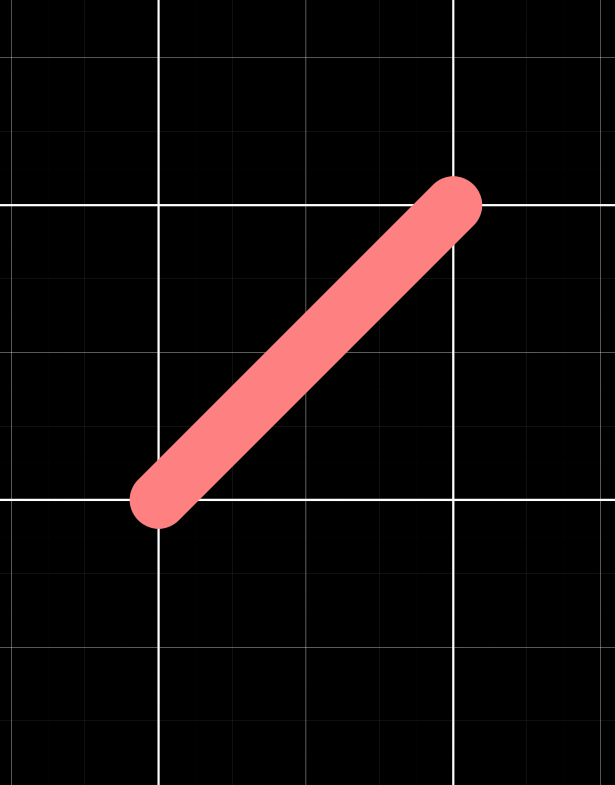
\includegraphics[width=0.2\textwidth]{fig/linie.png}
	\caption{Liniensegment}
	\label{fig:linie}
\end{figure}
\FloatBarrier


\subsection{Parallelogrammsegmente}
Eine andere Möglichkeit ist es Parallelogrammsegmente, wie in Abbildung \ref{fig:parallelogramm} zu nutzen.
\begin{figure}[ht]
	\centering
	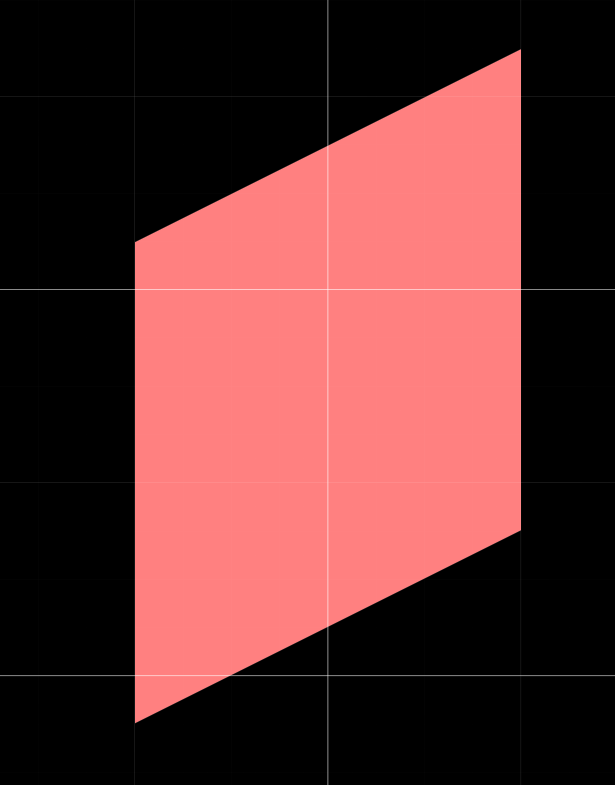
\includegraphics[width=0.2\textwidth]{fig/parallelogramm.png}
	\caption{Parallelogrammsegment}
	\label{fig:parallelogramm}
\end{figure}
\FloatBarrier

\subsection{Binärsuche}
\label{sec:binary}

